\documentclass[aspectratio=169]{beamer}
\usepackage{ctex,hyperref,amsmath,booktabs,array,graphicx}
\usepackage{SUFE}
\setbeamertemplate{navigation symbols}{}
\setbeamertemplate{headline}{}
\setbeamersize{text margin left=7mm,text margin right=7mm}
\setbeamerfont{frametitle}{size=\large}
\setbeamerfont{normal text}{size=\small}
\setbeamerfont{frame number}{parent=author in head/foot}
\title[深度特征选择与稳定性评价]{面向电商GMV监控的深度特征选择与稳定性评价研究}
\subtitle{相同样本扰动、双评价器与真实负结果}
\author{吴优\quad 2025213385}
\institute[上海财经大学]{上海财经大学统计与数据科学学院\\指导教师：张吕欧}
\date{2026年9月}
\begin{document}
\begin{frame}
\titlepage
\centering
\includegraphics[width=.19\linewidth]{pic/sufe.png}
\end{frame}
\begin{frame}{研究问题：有限容量的经营看板}
\begin{itemize}
\item 从31项经营指标中，选择值得持续监控的少量指标。
\item 预测任务提供信息保留标准；稳定性反映名单对卖家变化的敏感性。
\item 固定数量的推荐、原生错误控制和因果归因是不同问题。
\item 不预设复杂深度模型一定优于统计或树模型。
\end{itemize}
\end{frame}
\begin{frame}{真实文献与候选方法}
\small \begin{tabular}{lll}
\toprule
方法 & 年份 & 出处/角色\\\midrule
Deep Lasso & 2023 & NeurIPS D\&B；输入梯度正则\\
VTFS & 2024 & ACM TKDD；序列生成，定额适配\\
DeepDRK & 2024 & NeurIPS；深度Knockoff生成\\
TabM & 2025 & ICLR；参数高效集成\\
TabPFN v2 & 2025 & Nature；预训练表格模型\\
\bottomrule
\end{tabular}\vspace{0.5em}\begin{itemize}
\item 对照：Copula-MVR、Elastic Net、稳定性选择、影子树、XGBoost-SHAP。
\end{itemize}
\end{frame}
\begin{frame}{Olist数据与研究人口}
\begin{itemize}
\item 十张原始表：99,441条订单，112,650条商品明细。
\item 13,754个卖家月，2,723名卖家，18个特征月份。
\item 候选指标31项；本月有购买明细的卖家进入分析。
\item 下一月签收确认商品金额；不含运费，不等于利润或净收入。
\item 下一月目标为零的比例为17.8784\%。
\end{itemize}
\end{frame}
\begin{frame}{信息时间：月末只能使用已可见事件}
\begin{itemize}
\item 审核、承运、送达与评价按发生时间截断。
\item 营销成交按成交日期截断；州频率使用当时已观察卖家。
\item 支付、商品和卖家元数据缺少完整修订历史，仍有工作假设。
\item 预测选择不等于按品类、地区拆分当期GMV的会计贡献。
\end{itemize}
\end{frame}
\begin{frame}{时间切分与名单冻结}
\small \begin{tabular}{llr}
\toprule
阶段 & 目标月份 & 行数\\\midrule
训练 & 2017-02至2017-12 & 6,567\\
调参 & 2018-01至2018-02 & 1,831\\
排序 & 2018-03至2018-04 & 1,943\\
测试 & 2018-05至2018-07 & 3,413\\
\bottomrule
\end{tabular}\begin{itemize}
\item 测试前冻结主方法和K；预测器在全部开发数据重拟合。
\item 测试月份曾参与前期探索，不是全新外部确认样本。
\end{itemize}
\end{frame}
\begin{frame}{三种深度选择机制}
\begin{itemize}
\item Deep Lasso：训练时惩罚输入损失梯度，再按梯度分数排序。
\item TabM：训练8成员共享权重网络，再看验证集置换误差增量。
\item VTFS：从子集效用语料学习Transformer表示并搜索候选序列。
\item 三者都实际训练，但不自动获得FDR或因果解释。
\end{itemize}
\end{frame}
\begin{frame}{Deep Lasso：正则与输入选择}

\[
\mathcal L_{\mathrm{DL}}=\mathcal L_B+
\lambda\sum_j\|\partial\mathcal L_B/\partial X_{B,j}\|_2
\]
\begin{itemize}
\item 直接调用作者发布的正则函数，两层MLP，三个训练种子。
\item 验证早停；不使用测试集训练或选择检查点。
\item 补充去掉正则的同样本消融，检验当前配置下的局部作用。
\end{itemize}
\end{frame}
\begin{frame}{TabM：预测器与选择器分开评价}
\begin{itemize}
\item 官方2025年参数高效集成网络，8成员分别计算训练损失。
\item 每列置换3次，以MSE增加量形成排名。
\item 所有名单分别交给统一XGBoost与TabM重新预测。
\item 双评价器用于识别名单收益是否依赖特定预测模型。
\end{itemize}
\end{frame}
\begin{frame}{VTFS：适配与可解释的负结果}
\begin{itemize}
\item 使用官方编码器、解码器；96个随机子集语料。
\item 固定预算唯一token解码；效用查询不超过128次。
\item 保留公开代码中的常数重参数化，非完整原论文复现。
\item 完整样本最终名单来自语料回退，本次收益不能归功于解码器。
\end{itemize}
\end{frame}
\begin{frame}{公平稳定性：每种方法面对同一批卖家}
\begin{itemize}
\item 30组互补50\%样本，共60个半样本；卖家全部月份共同保留。
\item 20个70\%样本、20个80\%样本，共100个外层扰动。
\item 另有10组固定数据的种子诊断，与样本稳定性分开。
\item 比较K=4、8、10、12、14；主预算预设为12。
\item 50\%区间按30组计算，不把60个半样本视为独立。
\end{itemize}
\end{frame}
\begin{frame}{评价准则：各自回答不同问题}
\begin{itemize}
\item RMSE：保留的特征能否帮助下一期预测。
\item Jaccard：名单名称是否一致；Nogueira进行机会校正。
\item FDP：发现中假变量的比例；Power：真变量被找到的比例。
\item 真实业务没有已知真值，不能直接计算真实FDP。
\item 固定12项而只有5项真信号时，FDP至少为7/12。
\end{itemize}
\end{frame}
\begin{frame}{同样12项：测试预测结果}
\footnotesize \begin{tabular}{lrr}
\toprule
选择方法 & XGBoost RMSE & TabM RMSE\\\midrule
Copula-MVR & 1.8663 & 1.8945\\
Elastic Net & 1.8626 & 1.8737\\
稳定性选择 & 1.8931 & 1.8840\\
影子变量树 & 1.8606 & 1.8634\\
XGBoost-SHAP & 1.8464 & 1.8572\\
Deep Lasso & 1.8467 & 1.8600\\
TabM-置换 & 1.8443 & 1.8597\\
VTFS-定额适配 & 1.8625 & 1.8851\\
全维基线 & 1.8649 & 1.8588\\
\bottomrule
\end{tabular}\vspace{0.4em}\par\small 开发主选择VTFS未保持优势；TabM、Deep Lasso与树模型各有竞争力。
\end{frame}
\begin{frame}{相同卖家扰动：Top-12稳定性}
\footnotesize \begin{tabular}{lrrr}
\toprule
方法 & 50\% & 70\% & 80\%\\\midrule
Copula-MVR & 0.735 & 0.751 & 0.808\\
Elastic Net & 0.724 & 0.838 & 0.909\\
稳定性选择 & 0.583 & 0.662 & 0.702\\
影子变量树 & 0.939 & 0.962 & 0.992\\
XGBoost-SHAP & 0.768 & 0.847 & 0.822\\
Deep Lasso & 0.823 & 0.887 & 0.762\\
TabM-置换 & 0.750 & 0.878 & 0.893\\
VTFS-定额适配 & 0.407 & 0.481 & 0.297\\
\bottomrule
\end{tabular}\vspace{0.4em}\par\small 表中为相对完整开发名单的Jaccard；稳定性不等于正确率。
\end{frame}
\begin{frame}{展示容量：不能只看一条最有利结果}
\centering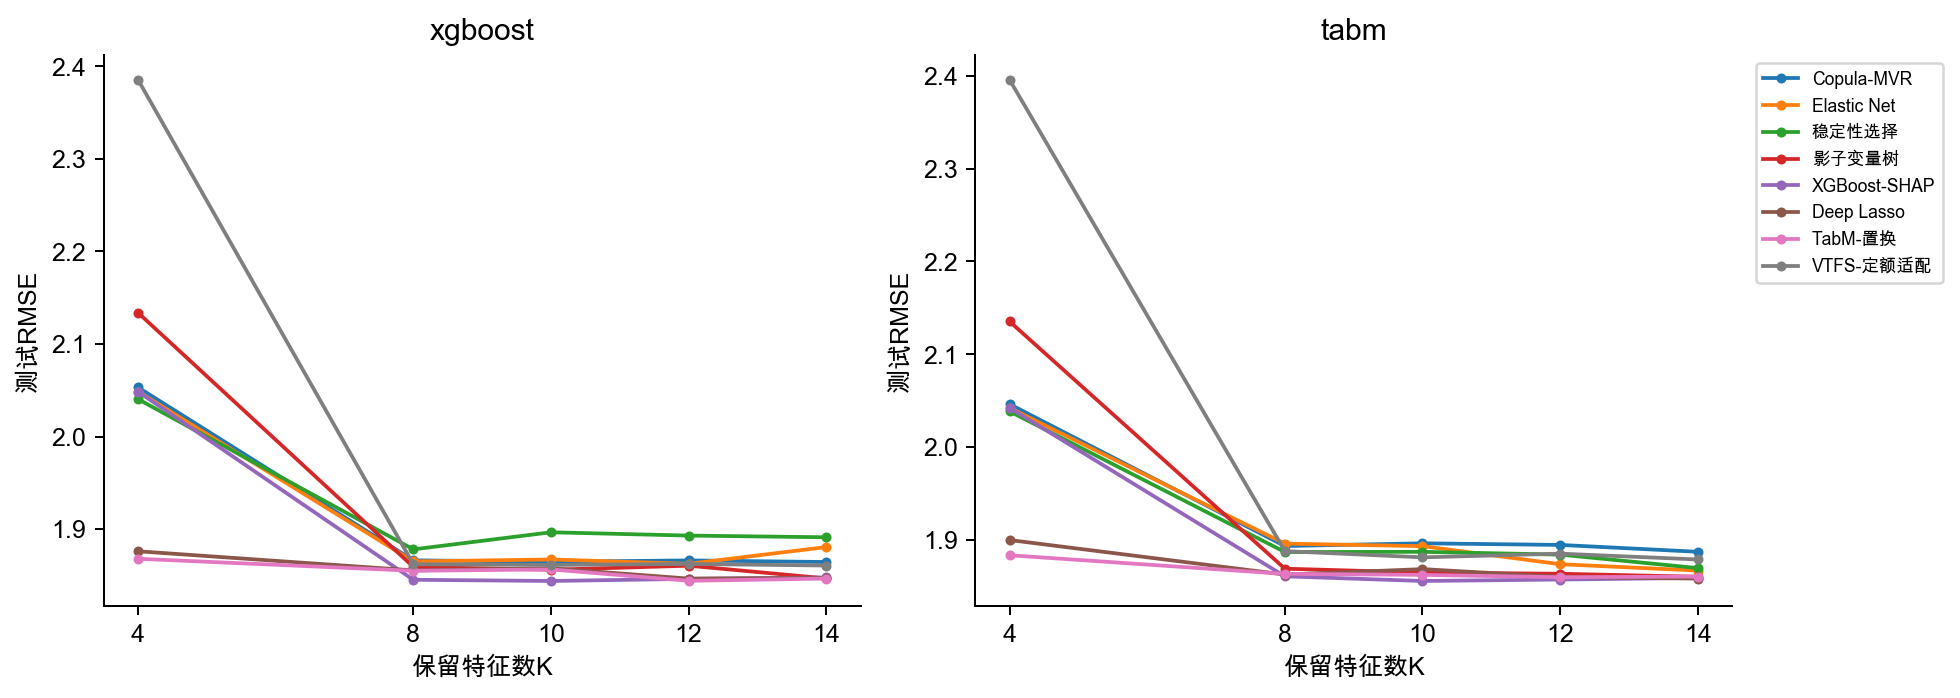
\includegraphics[width=.94\linewidth,height=.66\textheight,keepaspectratio]{figures/05_budget_path.png}\par\small VTFS按K=12优化顺序，其小K前缀不是独立优化结果。
\end{frame}
\begin{frame}{已知真值：每场景100次模拟}
\footnotesize \begin{tabular}{lrrrr}
\toprule
Top-12 Power & SHAP & D.Lasso & TabM & VTFS\\\midrule
线性稀疏强信号 & 1.000 & 1.000 & 1.000 & 0.776\\
线性中信号 & 0.991 & 0.996 & 0.997 & 0.561\\
线性弱信号 & 0.935 & 0.902 & 0.927 & 0.552\\
线性较密信号 & 0.782 & 0.793 & 0.799 & 0.485\\
非线性独立误差 & 0.964 & 0.831 & 0.843 & 0.585\\
非线性组内相关 & 0.970 & 0.846 & 0.823 & 0.567\\
\bottomrule
\end{tabular}\begin{itemize}
\item 全部八方法共享生成数据；完整FDP、Power和原生名单见论文。
\item 跨场景固定超参数，结果不代表各场景充分调参后的上界。
\end{itemize}
\end{frame}
\begin{frame}{生成诊断：不能无条件宣称真实FDR受控}
\centering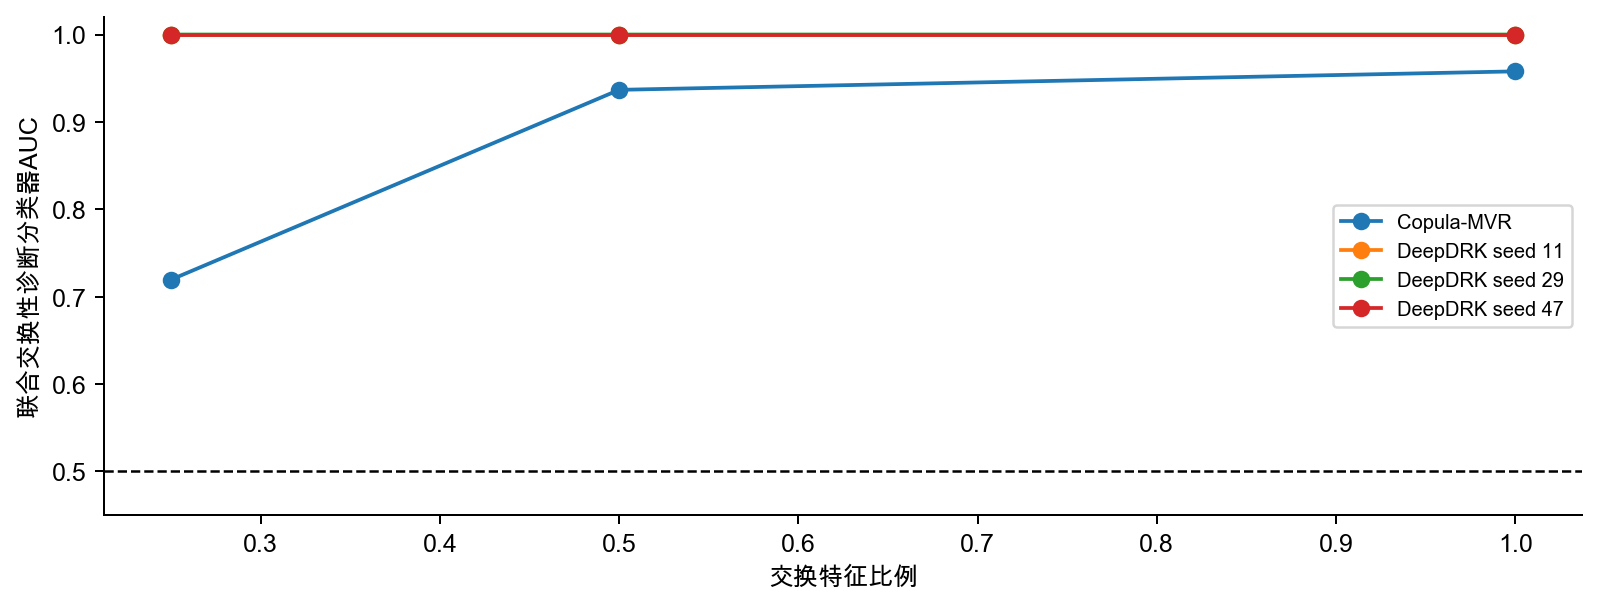
\includegraphics[width=.87\linewidth,height=.61\textheight,keepaspectratio]{figures/09_generator_diagnostic.png}\par\small Copula-MVR与DeepDRK均有联合失配警告；诊断不通过不等于反证原论文。
\end{frame}
\begin{frame}{负结果与局部消融}
\begin{itemize}
\item VTFS完整样本解码候选的开发效用增益为零，最终名单等于回退名单。
\item Deep Lasso保留/移除正则的半样本Jaccard：0.8230 / 0.8182；仅为固定配置消融。
\item DeepDRK只完成参考训练与诊断；TabPFN保留MPS失败记录。
\item 失败方法不填零、不补造结果，也不声称完成全部公平比较。
\end{itemize}
\end{frame}
\begin{frame}{结论与后续研究计划}
\begin{itemize}
\item 没有全面优胜者，深度结构复杂不等于名单质量更高。
\item 按新时间窗口验证TabM、Deep Lasso与强树基线。
\item 加强按K独立优化、等查询预算随机搜索和嵌套调参比较。
\item 研究混合变量与卖家依赖下的生成有效性，再讨论原生FDR。
\item 月度向周度迁移属于后续验证，不沿用未验证的多粒度结论。
\end{itemize}
\end{frame}
\begin{frame}{主要参考文献}
\begin{columns}[T]\begin{column}{.49\textwidth}\fontsize{6}{7.4}\selectfont[1] Cherepanova V, Levin R, Somepalli G, et al.. A Performance-Driven Benchmark for Feature Selection in Tabular Deep Learning. NeurIPS Datasets and Benchmarks Track, 2023.\par\vspace{0.4em}
[2] Ying W, Wang D, Chen H, Fu Y. Feature Selection as Deep Sequential Generative Learning. ACM Transactions on Knowledge Discovery from Data, 18(9), Article 221, 2024.\par\vspace{0.4em}
[3] Gorishniy Y, Kotelnikov A, Babenko A. TabM: Advancing Tabular Deep Learning with Parameter-Efficient Ensembling. International Conference on Learning Representations, 2025.\par\vspace{0.4em}
[4] Shen H, Yan Y, Zhao Z. DeepDRK: Deep Dependency Regularized Knockoff for Feature Selection. Advances in Neural Information Processing Systems, 2024.\par\vspace{0.4em}
[5] Hollmann N, Muller S, Purucker L, et al.. Accurate predictions on small data with a tabular foundation model. Nature, 637, 319-326, 2025.\par\vspace{0.4em}
[6] Candes E, Fan Y, Janson L, Lv J. Panning for gold: model-X knockoffs for high dimensional controlled variable selection. Journal of the Royal Statistical Society, Series B, 80(3), 551-577, 2018.\par\vspace{0.4em}
\end{column}\begin{column}{.49\textwidth}\fontsize{6}{7.4}\selectfont[7] Ren Z, Barber R F. Derandomised knockoffs: leveraging e-values for false discovery rate control. Journal of the Royal Statistical Society, Series B, 86(1), 122-154, 2024.\par\vspace{0.4em}
[8] Wang R, Ramdas A. False discovery rate control with e-values. Journal of the Royal Statistical Society, Series B, 84(3), 822-852, 2022.\par\vspace{0.4em}
[9] Meinshausen N, Buhlmann P. Stability selection. Journal of the Royal Statistical Society, Series B, 72(4), 417-473, 2010.\par\vspace{0.4em}
[10] Shah R D, Samworth R J. Variable selection with error control: another look at stability selection. Journal of the Royal Statistical Society, Series B, 75(1), 55-80, 2013.\par\vspace{0.4em}
[11] Nogueira S, Sechidis K, Brown G. On the Stability of Feature Selection Algorithms. Journal of Machine Learning Research, 18(174), 1-54, 2018.\par\vspace{0.4em}
[12] Morris T P, White I R, Crowther M J. Using simulation studies to evaluate statistical methods. Statistics in Medicine, 38(11), 2074-2102, 2019.\par\vspace{0.4em}
\end{column}\end{columns}\vfill{\scriptsize 完整26项来源及可访问链接见论文参考文献。}
\end{frame}
\end{document}
